%!TEX root = ../thesis.tex
This section will focus on describing and discussing a selection of concepts for ad hoc interfaces based on the jamming technique.
As mentioned in the beginning of this chapter we were not successful at implementing a working jamming system where we could control air/liquid flow. \todo{make sure this is actually addressed. Suggestions: complexity, price of equipment: mechanics is one thing, the other is materials, i.e. ecoflex rubber etc.}
Therefore we concentrate on conceptual prototypes which we envisioned before taking the decision to move in other directions.
Each of these concepts have different focal points.
The first one, \emph{ \nameref{ch:jamming:concepts:dynamic_input} }, strives to achieve on-demand standard interfaces for input control.
The second, \emph{ \nameref{ch:jamming:concepts:playful_blobs} }, seeks to draw on known interaction metaphors from the digital world and  expose them to physical objects.
The third, \emph{ \nameref{ch:jamming:concepts:improvised_furniture} }, scales up the dimensions and focuses on a living environment with highly configurable components.
\blank
\todo{Afsnit hvor der n\o gternt bliver redegjort for kompleksiteten og vores misl\o kkede fors\o g.}

\subsection{Dynamic input controls} 
\label{ch:jamming:concepts:dynamic_input}

\todo{what's the problem with static dashboards}\\

Cell-based jamming, as mentioned in \ref{ch:jamming}, allows for deformations of individual cells.
This technique \hl{opens up} for a new and very dynamic approach to inputs, such as buttons, knobs, etc.
These input controls could emerge from the otherwise flat surface when needed, see figure~\ref{fig:ch:jamming:concepts:button}.
Other than being able to hide input controls when not needed this approach also opens up for a configurable interface adapted to a specific user's preference.
\citet{harrison2009providing} (\citeyear{harrison2009providing}) have previously made a contribution to physically changeable visual displays.
Their approach is not based on jamming but also on a pneumatic actuation which allow deformations of a latex surface.
This approach makes it possible to programmatically modify input control between three states: positive, neutral and negative, see figure~\ref{fig:ch:jamming:concepts:harrisonhudson}.
Though input controls are deformable and have tactile qualities, the displays are still in a very static configuration.
The positioning and shape of input controls are based on a acrylic backing layer with cut-out areas which cannot be changed.

\begin{figure}[h]
  \centering
      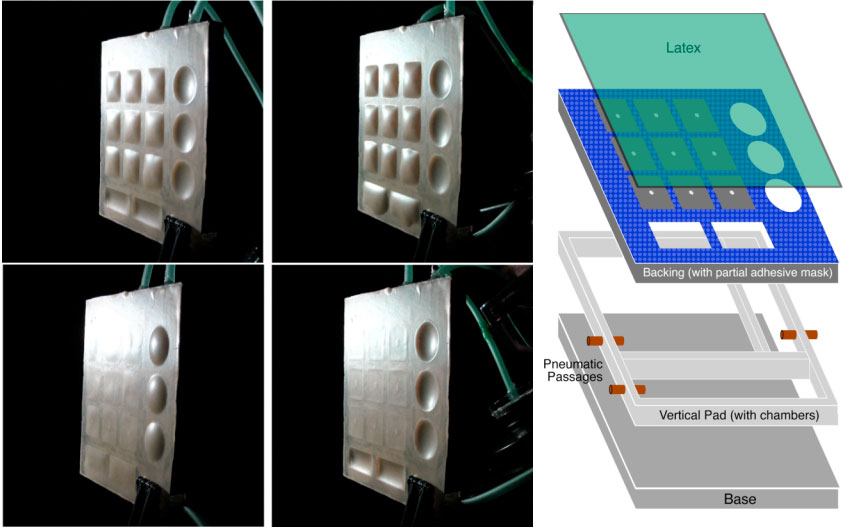
\includegraphics[width=.8\textwidth]{figures/jamming/concepts/harrisonhudson}
  \caption[A tactile display in various interfaces states. All buttons are statically positioned.]
  {A tactile display in various interfaces states. All buttons are statically positioned.}
  \label{fig:ch:jamming:concepts:harrisonhudson}
\end{figure}

\begin{figure}
  \centering
      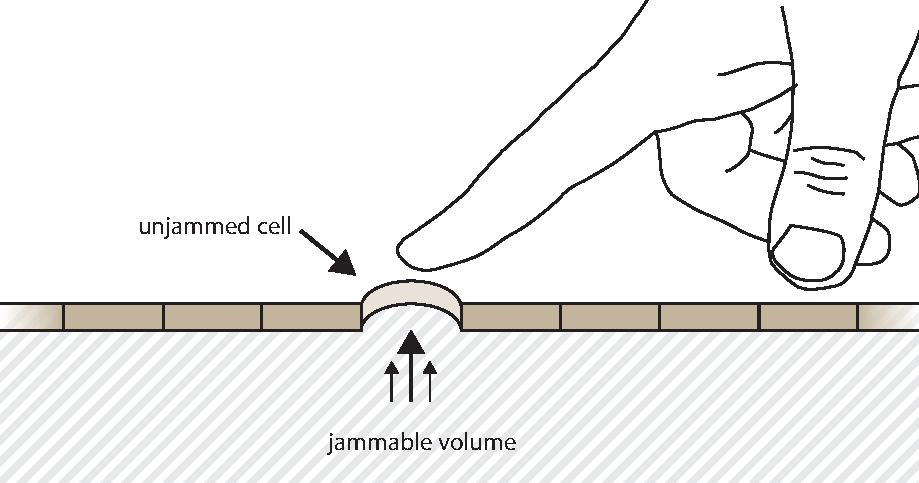
\includegraphics[width=3in]{figures/jamming/concepts/jamming_button}
  \caption[A cell-based jammable button.]
  {A cell-based jammable button.}
  \label{fig:ch:jamming:concepts:button}
\end{figure}

We conceptualize on household appliances such as radios, clock alarms, house alarms heating, ventilation and air conditioning (HVAC), \todo{etc}.
In general physical products with standard input controls such as buttons, knobs, switches and sliders.

\subsection{Playful blobs}
\label{ch:jamming:concepts:playful_blobs}

The focal point of this next concept is on bringing input and output into the same object.
As can be seen in table~\ref{ch:jamming:table:applications_overview} on page~\pageref{ch:jamming:table:applications_overview} only one of the listed projects from the related work section have both input and output in same object. \todo{what does that say?}

\nameref{ch:jamming:concepts:playful_blobs} is a toy concept for children.
The blobs are tangible clay-like objects meant to be molded into creative forms.
Each blob makes a selection of commands available otherwise known from digital interface metaphors, such as \emph{save, open, undo, delete, copy, and paste} which can actuate the blob in different ways.
These commands give a physical blob a notion of form memory where state is kept over time.
More specifically each command means (see also figure~\todo{ref}:
\begin{itemize}
	\item{\emph{Save}: The current form of a blob is saved in memory for later retrieval.}
	\item{\emph{Open}: A previously saved form can be recalled and the blob actuates itself into the saved state.}
	\item{\emph{Undo}: Negate the latest molding of the form.}
	\item{\emph{Copy}: Make a copy of the state of a specific blob. The copied state could be saved in a blob or in an external object.}
	\item{\emph{Paste}: Set the state of a blob to that of which has been copied.} 
	\item{\emph{Delete}: Reset a blob so that all state is forgotten.} 
\end{itemize}
The commands are made possible via a cell-based jamming structure.
As mentioned earlier this jamming approach makes it possible to separately control the stiffness of each cell.
So, for example, the \emph{save} command is done by storing a map of the current pressure states of each cell.
A subsequent \emph{open} or \emph{paste} command would set the correct pressure values of the cells and thereby restore the \emph{saved} or \emph{copied} physical form.
Lastly, a \emph{delete} command would release all negative pressure in cells and thereby collapse the form.

Applying these digital features to the physical blobs brings about ad hoc qualities.
If needed previously saved forms can be recalled and further work on the form can done.

The amount of detail a molded blob can have is dictated by the resolution of the jamming cells.
\blank
\todo{ad hoc qualities \dots}
\begin{verbatim}
tool tankegang. bringe en gammel form frem.
digitale kvaliteter der overfoeres. arbejde videre paa formen. formsprog
gengive forloebet formgivningen.
den rigtige jamming raekkefoelge
\end{verbatim}

\subsection{Improvised furniture}
\label{ch:jamming:concepts:improvised_furniture}

This concept is based on replacing static components of the home with dynamic jamming enabled substitutes.
In its most extreme case with a large scale deployment it may be a little far fetched but not unrealistic in a more futuristic scenario.
It underpins the idea of a configurable home where otherwise static and massive components such as walls and furniture allow for deformations.
For example, \todo{pushing in} part of a wall to make room for a plant or even an entire shelf.
Or, deforming the floor to improvise an extra seat for a guest.
With this reconfigurability done by hand the components will naturally end up having an organic appearance with curvatures and very few straight lines and edges giving.

Using jamming in a large scale deployment where strength and bearing capacity is a requirement does come with quite a few constraints regarding materials.
The container of the particles must be strong enough to handle the exposed level of stress and strain while still being flexible enough to allow for surface deformations.

\begin{verbatim}
1. dynamisk input kontrol
2. input + output kombination - ishii + rund robot (standard verbs)
	copy, paste, undo, delete form - digitale -> fysiske verden.
3. improviseret moebler (det fuldstaendig modelerbare hjem - tanken om at man kan tage selve strukturen af huset ned paa et niveau hvor man kan aendre i hoejere grad.)

\end{verbatim}

